% Giles (2000) has a good discussion on this.
% \cite{ma_comparison_2021}. 

In this section we are going to address how these tools are computationally implemented and how to decide which method to use depending the problem. 
This decision is in general driven by the type of differential equation (stiff or non-stiff, number of equations, number of parameters) and the available computational resources. 
The most important considerations that modern software needs to deal with in order to compute sensitivities are 
\begin{enumerate}
    \item How to handle matrix/Jacobian-vector products
    \item Numerical stability
    \item Memory and runtime tradeoff
\end{enumerate}
This considerations also vary depending if the sensitivity method directly depends of the differential equation and the numerical solver used to solve it or if instead the gradient is compute independently of the internals of the solver. 


\subsection{Solver-free methods}

Let us start comparing how finite differences and complex-step differentiation perform for a simple problem with one single parameter. 
Figure \ref{fig:finite-diff} illustrates the error in computing the gradient of a simple loss function for both true analytical solution and numerical solution of a system of ODEs as a function of the stepsize $\varepsilon$.

\begin{figure}[tbh]
    \centering
    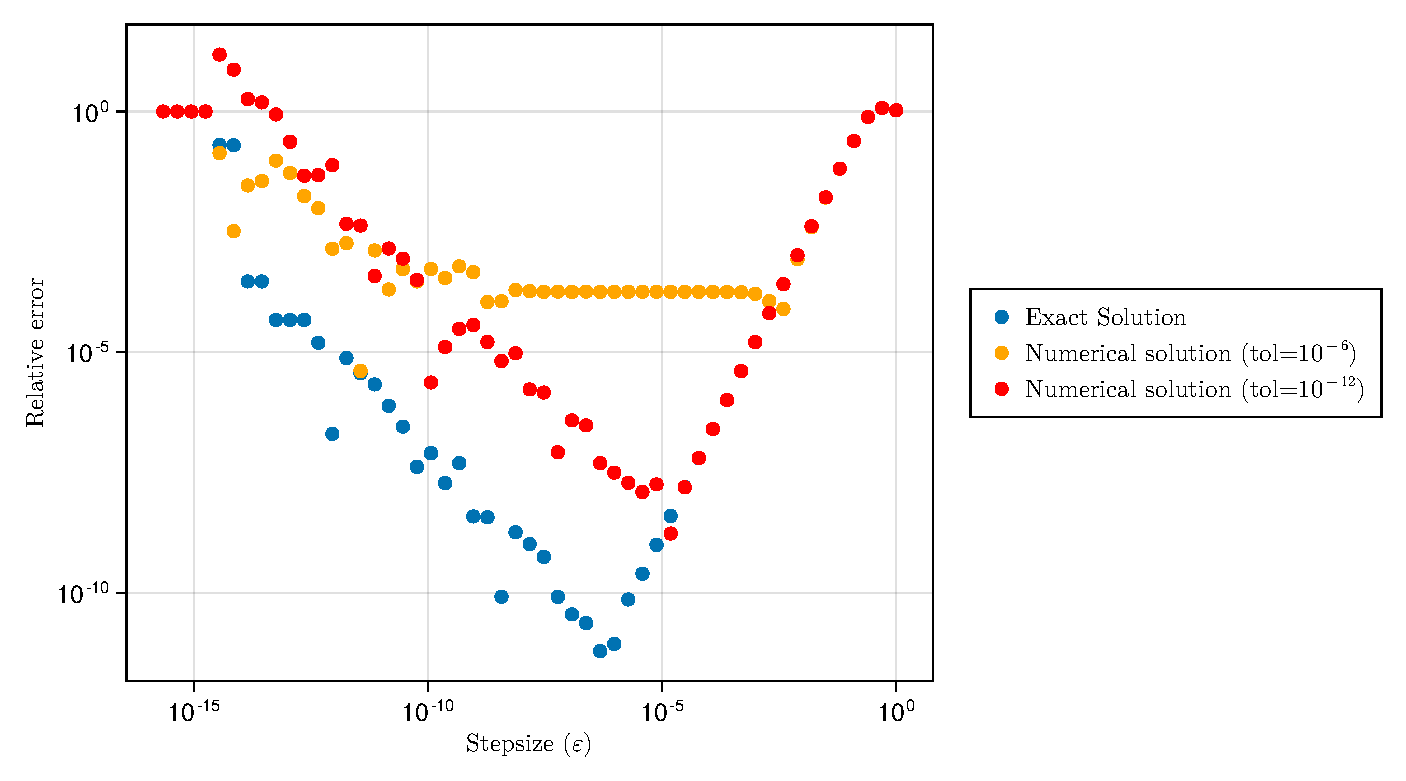
\includegraphics[width=0.85\textwidth]{../code/finite_differences/finite_difference_derivative.pdf}
    \caption{Absolute relative error when computing the gradient of the function $u(t) = \sin (\omega t)/\omega$ with respect to $\omega$ at $t=10.0$ as a function of the stepsize $\varepsilon$. Here $u(t)$ corresponds to the solution of the differential equation $u'' + \omega^2 u = 0$ with initial condition $u(0)=0$ and $u'(0)=1$. The blue dots correspond to the case where this is computed finite differences. The red and orange lines are for the case where $u(t)$ is numerically computed using the default Tsitouras solver \cite{Tsitouras_2011} from \texttt{OrdinaryDiffEq.jl} using different tolerances. The error when using  a numerical solver is larger and it is dependent of the numerical precision of the numerical solver. }
    \label{fig:finite-diff}
\end{figure}

In general, finite differences is very easy to implement since it does not require any type of software support, but it is a less accurate and as costly as forward AD \cite{Griewack-on-AD} and comple-step differentiation. 
Implementing these last types in a programming language implies defining what it means to perform basic operations and then combine them using the chain rule provided by the dual number properties.
In Julia we can create a dual number by defining an object with two values, and then extend the definition of algebraic operations and functions, a process known as \textit{operator overloading} \cite{Neuenhofen_2018}, by relying in multiple dispatch:
\begin{jllisting}
using Base: @kwdef

@kwdef struct DualNumber{F <: AbstractFloat}
    value::F
    derivative::F
end

# Binary sum
Base.:(+)(a::DualNumber, b::DualNumber) = DualNumber(value = a.value + b.value, derivative = a.derivative + b.derivative)

# Binary product 
Base.:(*)(a::DualNumber, b::DualNumber) = DualNumber(value = a.value * b.value, derivative = a.value*b.derivative + a.derivative*b.value)
\end{jllisting}
and then we can simply evaluate derivatives by evaluating the derivative component of the dual number that results from the combination of operations
\begin{jllisting}
a = DualNumber(value=1.0, derivative=1.0)

b = DualNumber(value=2.0, derivative=0.0)
c = DualNumber(value=3.0, derivative=0.0)

result = a * b * c
println("The derivative of a*b*c with respect to a is: ", result.derivative)
\end{jllisting}
Notice that in this last example the dual numbers \texttt{b} and \texttt{c} where initialized with derivative value equals to zero, while \texttt{a} with value equals to one. 
This is because we were interested in computing the derivative with respect to \texttt{a}, and then $\frac{\partial a}{\partial a} = 1$, while $\frac{\partial b}{\partial a} = \frac{\partial c}{\partial a} = 0$. 

We can also extend the definition of standard functions by simply applying the chain rule and storing the derivative in the dual variable following Equation \eqref{eq:dual-number-function}:
\begin{jllisting}
function Base.:(sin)(a::DualNumber)
    value = sin(a.value)
    derivative = a.derivative * cos(a.value)
    return DualNumber(value=value, derivative=derivative)
end
\end{jllisting}
With all these pieces together, we are able to propagate forward the value of a single-valued derivative though a series of algebraic operations. 

In the Julia ecosystem, \texttt{ForwardDiff.jl} implements forward mode AD with multidimensional dual numbers \cite{RevelsLubinPapamarkou2016}. 
Notice that a major limitation of the dual number approach is that we need a dual variable for each variable we want to differentiate. 
Implementations of forward AD using dual numbers and computational graphs require a number of operations that increases with the number of variables to differentiate, since each computed quantity is accompanied by the corresponding gradient calculations \cite{Griewack-on-AD}. 
This consideration applies to most forward methods. 

Notice that both AD based in dual number and complex-step differentiation are based on defining and extended variable that carries information about the gradient. 
% Another important point of comparison is the one existing between forward mode AD implemented with dual numbers and complex step differentiation. 
Both methods introduce an abstract unit ($\epsilon$ and $i$, respectively) associated to the imaginary part of the extender value that carries forward the numerical value of the gradient. 
This resemblance between the methods makes them to be susceptible to the same advantages and disadvantages: easiness to implement with operator overloading; inefficient scaling with respect to the number of variables to differentiate. 
However, although these methods seems very similar, it is important to remark that AD gives the exact gradient, while complex step differentiation relies in numerical approximations that are valid just when the stepsize $\varepsilon$ is small. 
The next example shows how the calculation of the gradient of $\sin (x^2)$ is performed by these two methods:
\begin{equation}
\renewcommand{\arraystretch}{1.5}
\begin{tabular}{@{} l @{\qquad} l @{\qquad} l @{}}
Operation & AD with Dual Numbers  & Complex Step Differentiation \\
$x$ & $x + \epsilon$    & $x + i \varepsilon$ \\
$x^2$ & $x^2 + \epsilon \, (2x)$  & $x^2 - \varepsilon^2 + 2i\varepsilon x$\\
$\sin(x^2)$  & $\sin(x^2) + \epsilon \, \cos(x^2) (2x)$ &
$\sin(x^2 - \varepsilon^2) \cosh (2i\varepsilon) + i \, \cos(x^2 - \varepsilon^2) \sinh (2i\varepsilon)$
\end{tabular}
\label{eq:AD-complex-comparision}
\end{equation}
While the second component of the dual number has the exact derivative of $\sin(x^2)$, it is not until we take $\varepsilon \rightarrow 0$ than we obtain the derivative in the imaginary component for the complex step method
\begin{equation}
    \lim_{\varepsilon \rightarrow 0} \, \frac{1}{\varepsilon} \, \cos(x^2 - \varepsilon^2) \sinh (2i\varepsilon) 
    = 
    \, \cos(x^2) (2x).
\end{equation}
The stepsize dependence of the complex step differentiation method makes it resemble more to finite differences than AD with dual numbers. 
This difference between the methods also makes the complex step method sometimes more efficient than both finite differences and AD \cite{Lantoine_Russell_Dargent_2012}, an effect that can be counterbalanced by the number of extra unnecessary operation that complex arithmetic requires (see last column of \eqref{eq:AD-complex-comparision}) \cite{Martins_Sturdza_Alonso_2003_complex_differentiation}.

\subsubsection{Backpropagation}

The libraries \texttt{ReverseDiff.jl} and \texttt{Zygote.jl} use callbacks to compute gradients. When gradients are being computed with less than $\sim 100$ parameters, the former is faster (see documentation).

\subsection{Solver-based methods}

Just a few modern scientific software have the capabilities of handling ODE solvers and compute their sensitivities at the same time. 
The include \texttt{CVODES} within \texttt{SUNDIALS} in C \cite{serban2005cvodes, SUNDIALS-hindmarsh2005sundials}; \texttt{ODESSA} \cite{ODESSA} and \texttt{FATODE} \cite{FATODE2014} both in Fortram; \texttt{SciMLSensitivity.jl} in Julia \cite{rackauckas2020universal}; \texttt{Dolfin-adjoint} based on the \texttt{FEniCS} Project \cite{dolfin2013, dolfin2018}. 
On the other hand, it is important to remark that the underlying machinery of all solvers relies in solvers for linear systems of equations, which can be solved in dense, band (sparse) and Krylow mode. 
This implies that methods based on numerical solvers are, in principle, more difficult to implement but also more efficient in computing gradients for complex differential equations. 
Another important consideration is that all these methods have subroutines to compute the VJPs involved in the sensitivity and adjoint equations. 
This calculation is carried by another sensitivity method (finite differences, AD) and this also plays a central role at the moment of analyzing accuracy and stability of the adjoint method. 

\subsubsection{Sensitivity equation}

\subsubsection{Solving the adjoint}

An equal important consideration when working with adjoints is when these are numerically stable. 
Some works had shown that continuous adjoints can lead to unstable sensitivities \cite{Jensen_Nakshatrala_Tortorelli_2014}.
Implicit forward schemes can give rise to explicit backwards schemes, leading to unstable solutions for the gradient. 

\vspace*{10px}
\noindent \textbf{\textit{Solving the backwards mode}}
\vspace*{5px}

The bottleneck on this method is the calculation of the adjoint, since in order to solve the adjoint equation we need to know $u(t)$ at any given time. 
Effectively, notice that the adjoint equation involves the term $f(u, \theta, t)$ and $\frac{\partial h}{\partial u}$ which are both functions of $u(t)$. 
There are different ways of addressing the evaluation of $u(t)$ during the backwards step.
\begin{enumerate}[label=(\roman*)]
    \item \textbf{Dense Store.} During the forward model, we can just store in memory all the intermediate states of the numerical solution. 
    This leads to heavy-memory expensive algorithms. 
    \item \textbf{Re-solve.} Solve again the original ODE together with the adjoint as the solution of the reversed augmented system \cite{chen_neural_2019}
    \begin{equation}
    \frac{d}{dt}
    \begin{bmatrix}
       u \\
       \lambda \\
       \frac{dL}{d\theta}
    \end{bmatrix}
    = 
    \begin{bmatrix}
       -f \\
       - \frac{\partial f}{\partial u}^T \lambda - \frac{\partial h}{\partial u}^T \\
       - \lambda^T \frac{\partial f}{\partial \theta} - \frac{\partial h}{\partial \theta}
    \end{bmatrix}
    % = 
    % - [ 1, \lambda^T, \lambda^T ]
    % \begin{bmatrix}
    %    f & \frac{\partial f}{\partial u} & \frac{\partial f}{\partial \theta} \\
    %    0 & 0 & 0 \\
    %    0 & 0 & 0
    % \end{bmatrix},
    \qquad 
    \begin{bmatrix}
       u \\
       \lambda \\
       \frac{dL}{d\theta}
    \end{bmatrix}(t_1)
    = 
    \begin{bmatrix}
       u(t_1) \\
       \frac{\partial L}{\partial u(t_1)} \\
       \lambda(t_0)^T s(t_0)
    \end{bmatrix}.
    \end{equation}
    However, computing the ODE backwards can be unstable and lead to large numerical errors \cite{kim_stiff_2021, Zhuang_2020}. 
    \item \textbf{Checkpointing. } Also known as windowing, ckeckpointing is a technique that trade-offs memory and time by saving intermediate states of the solution in the forward pass and recalculating the solution between intermediate states in the backwards mode \cite{Checkpoiting_2023, griewank2008evaluatingderivatives}. 
    This is implemented in \texttt{Checkpointing.jl} \cite{Checkpoiting_2023}.
\end{enumerate} 

One way of solving this system of equations that ensures stability is by using implicit methods. 
However, this requires cubic time in the total number of ordinary differential equations, leading to a total complexity of $\mathcal O((n+p)^3)$ for the adjoint method.
Two alternatives are proposed in \cite{kim_stiff_2021}, the first one called \textit{Quadrature Adjoint} produces a high order interpolation of the solution $u(t)$ as we move forward, then solve for $\lambda$ backwards using an implicit solver and finally integrating $\frac{dL}{d\theta}$ in a forward step.
This reduces the complexity to $\mathcal O (n^3 + p)$, where the cubic cost in the number of ODEs comes from the fact that we still need to solve the original stiff differential equation in the forward step. 
A second but similar approach is to use a implicit-explicit (IMEX) solver, where we use the implicit part for the original equation and the explicit for the adjoint. 
This method also will have complexity $\mathcal O (n^3 + p)$.

\vspace*{10px}
\noindent \textbf{\textit{Solving the quadrature}}
\vspace*{5px}

Another computational challenge in the computation of the continuous adjoint is how the integral in Equation \eqref{eq:casa-final-loss-gradient} is numerically evaluated. 
Some methods save computation by noticing that the last step in the continuous adjoint method of evaluating $\frac{dL}{d\theta}$ is an integral instead of a ODE, and then can be evaluated as such without the need of including it in the tolerance calculation inside the numerical solver \cite{that-is-not-an-ode}.
Numerical solutions of the integral 
\begin{equation}
    \int_{t_0}^{t_1} 
    \approx
    \sum 
\end{equation}
Gaussian quadrature is the faster method to evaluate one-dimensional integrals \cite{Norcliffe_gaussquadrature_2023}.

Weights and knots are obtained in order to maximize the order of which polynomials are exactly integrated \cite{stoer2002-numerical}    . 

\subsubsection{Further considerations}

In SUNDIALS, the VJPs involved in the sensitivity and adjoint method are handled using finite differences unless specified by the user \cite{SUNDIALS-hindmarsh2005sundials}.